% GENERATED by harness/assemble_contract.py --all; do not edit.
\section*{Main results, module by module}
\noindent Each contract's main results, the modules in dependency order (a module after every module it builds on). A heading opens the statement in its contract.

\subsection*{\href{../modules/foundations/contract.pdf}{Foundations: quantum-information preliminaries, number model, exact admissibility and emission}}
\noindent{\small version 0.12.0, \href{../modules/foundations/digest.pdf}{statements digest}}\par\smallskip
\par\medskip\noindent\textbf{\hyperref{../modules/foundations/contract.pdf}{}{claim-foundations/lem:kernel}{Lemma~1.4 (Extended divergence kernel)}}\par\nopagebreak\noindent The divergence kernel d(u, v) = u log\ensuremath{_{2}}(u/v), extended to vanishing arguments, is jointly convex, lower semicontinuous and non-increasing in v. These properties keep the objective well defined at support boundaries and let it be composed with concave branch quantities.
\par\medskip\noindent\textbf{\hyperref{../modules/foundations/contract.pdf}{}{claim-foundations/lem:pinchmono}{Lemma~1.5 (Pinching lowers the trace power)}}\par\nopagebreak\noindent For \ensuremath{\alpha} \textgreater{} 1, pinching the \ensuremath{\alpha}-th root of a positive semidefinite operator and raising the result to the power \ensuremath{\alpha} never increases the trace, and leaves it unchanged exactly when the operator is block diagonal for the pinching. This bounds the trace-power terms of the MEAT objective.
\par\medskip\noindent\textbf{\hyperref{../modules/foundations/contract.pdf}{}{claim-foundations/lem:exact-accumulation}{Lemma~3.4 (Exactness of a sum that rounds nowhere)}}\par\nopagebreak\noindent A sequential sum rounds nowhere exactly when every exact partial sum is a binary64 number, and then the computed sum equals the exact sum at every step. A predicate stated on such a sum is a predicate on the declared values themselves.
\par\medskip\noindent\textbf{\hyperref{../modules/foundations/contract.pdf}{}{claim-foundations/def:exact-admissibility}{Definition~4.3 (Exact admissibility of a declared operator family)}}\par\nopagebreak\noindent A declared operator family is exactly admissible for a sector map with constant c when (T) its own sector map agrees, (H) every block is exactly Hermitian, (P) positive, (C) it sums to c times the identity and (S) its declared-order sum rounds nowhere. Each is a property of the declared numbers.
\par\medskip\noindent\textbf{\hyperref{../modules/foundations/contract.pdf}{}{claim-foundations/req:boundary-admission}{Requirement~9.1 (Exact admissibility at every module boundary)}}\par\nopagebreak\noindent Declared operator data cross every module boundary exactly admissible, so every sum a predicate reads is the exact sum. The declarer makes them so, or, for data an instance passes on unchanged, the consumer's exact decision on entry does, and a consumer that finds otherwise refuses them.

\subsection*{\href{../modules/receiver/contract.pdf}{Receiver POVM (receiver)}}
\noindent{\small version 0.11.0, \href{../modules/receiver/digest.pdf}{statements digest}}\par\smallskip
\par\medskip\noindent\textbf{\hyperref{../modules/receiver/contract.pdf}{}{claim-receiver/thm:click-povm}{Theorem~4.5 (Click-pattern POVM)}}\par\nopagebreak\noindent The click patterns of a receiver instrument form a POVM whose elements follow from the port Grams by inclusion and exclusion. Every element is block diagonal in the total input photon number, and vacuum gives only the no-click outcome.
\par\medskip\noindent\textbf{\hyperref{../modules/receiver/contract.pdf}{}{claim-receiver/thm:coarse-graining}{Theorem~5.6 (Coarse-graining of the click-pattern POVM)}}\par\nopagebreak\noindent The emitted POVM of a declared coarse-graining is a POVM, block diagonal in the photon number, and lower bounds on disjoint raw outcomes add. A bound on a merged outcome gives nothing about the click patterns it merges.
\par\medskip\noindent\textbf{\hyperref{../modules/receiver/contract.pdf}{}{claim-receiver/thm:emitted-bound}{Theorem~8.14 (Multiclick bounds carried by the emitted weights)}}\par\nopagebreak\noindent Each setting's emitted weight bounds its multiclick element on every photon-number block above the cutoff, and their minimum does so at every setting, under the eigenvalue-slack assumption \hyperref{../modules/receiver/contract.pdf}{}{claim-receiver/ass:eig}{A-EIG} only where computed block eigenvalues enter. Each weight lies in [0, 1] and is finitely computable.
\par\medskip\noindent\textbf{\hyperref{../modules/receiver/contract.pdf}{}{claim-receiver/prop:slotvalid}{Proposition~8.17 (Range of the strengthening-slot weights)}}\par\nopagebreak\noindent At every setting the strengthening slot's weights (high-photon lower bounds on disjoint sets of raw outcomes) are non-negative and sum to at most one, as are their minima over the settings, and each emitted multiclick weight lies in [0, 1]. That the emitted weights are valid bounds is \hyperref{../modules/receiver/contract.pdf}{}{claim-receiver/thm:emitted-bound}{Theorem~8.14}.
\par\medskip\noindent\textbf{\hyperref{../modules/receiver/contract.pdf}{}{claim-receiver/component-catalogue/thm:catalogue-admissibility}{Theorem~16.3 (Admissibility of the catalogue entries)}}\par\nopagebreak\noindent Every catalogue entry maps its whole declared parameter domain to contractions on its modes, lossless exactly on the subfamily the catalogue's table lists for it. Only the generic block, an arbitrary matrix on declared modes, needs its contractivity checked at admission.
\par\medskip\noindent\textbf{\hyperref{../modules/receiver/contract.pdf}{}{claim-receiver/detector-imperfections/thm:efficiency}{Theorem~18.1 (Detector efficiency in the port Grams)}}\par\nopagebreak\noindent Efficiency \ensuremath{\eta}\_k uniform on detector port k scales that port's Gram by \ensuremath{\eta}\_k, keeping its rank if \ensuremath{\eta}\_k \textgreater{} 0; varying within a port, it is no scalar and can lower the rank. It enters only as the compiled instrument matrix's last layer, and the loss decomposition \hyperref{../modules/receiver/contract.pdf}{}{claim-receiver/lem:deficiency}{Lemma~4.2} checks that loss is counted once.
\par\medskip\noindent\textbf{\hyperref{../modules/receiver/contract.pdf}{}{claim-receiver/detector-imperfections/thm:dark-counts}{Theorem~19.2 (Dark counts on a photon-number block-diagonal POVM)}}\par\nopagebreak\noindent A dark-count channel keeps the photon-number block-diagonal POVM structure and never moves weight out of the multiclick set. It raises the multiclick bound p\_mc to (1 \ensuremath{-} r\_min)p\_mc + r\_min, where r\_min is the least multiclick mass over every non-multiclick column, the no-click column included.

\subsection*{\href{../modules/transmitter/contract.pdf}{Transmitter source model (transmitter)}}
\noindent{\small version 0.13.0, \href{../modules/transmitter/digest.pdf}{statements digest}}\par\smallskip
\par\medskip\noindent\textbf{\hyperref{../modules/transmitter/contract.pdf}{}{claim-transmitter/lem:ensemble-presentation}{Lemma~3.4 (Certificate defined by an ensemble presentation)}}\par\nopagebreak\noindent A virtual ensemble in sector blocks defines, by canonical purification and a square-root measurement, a block certificate with pure blocks that exactly reproduces Alice's marginal and, under that measurement, the ensemble. Only her marginal, a transposed sum of declared blocks, is formed as numbers.
\par\medskip\noindent\textbf{\hyperref{../modules/transmitter/contract.pdf}{}{claim-transmitter/thm:certificate-sufficiency}{Theorem~4.1 (Checkability and sufficiency of the source-replacement certificate)}}\par\nopagebreak\noindent In any form (pure projector, sector blocks, ensemble presentation) the certificate's algebraic conditions are finitely many exact decisions making Alice's measurement reproduce the virtual ensemble. Under retention and sequential rounds she may measure before or after any attack: source replacement.
\par\medskip\noindent\textbf{\hyperref{../modules/transmitter/contract.pdf}{}{claim-transmitter/lem:matched-pinching}{Lemma~4.5 (Matched pinching of a block certificate)}}\par\nopagebreak\noindent A block certificate is unchanged by pinching Alice's sectors or the virtual signal's sectors paired with them, so every state an admitted attack reaches from it is block diagonal with Alice's declared marginal. An operator merely constrained to have that marginal need not be block diagonal.
\par\medskip\noindent\textbf{\hyperref{../modules/transmitter/contract.pdf}{}{claim-transmitter/decoy/prop:tagging}{Proposition~8.1 (Tagging channel for weights at or below the Poisson weights)}}\par\nopagebreak\noindent One channel, independent of the label, maps each tagged virtual state to its phase-randomised weak coherent state whenever the declared sector weights lie at or below the Poisson weights. The weights therefore need only a certified inequality, never an exact Poisson weight.
\par\medskip\noindent\textbf{\hyperref{../modules/transmitter/contract.pdf}{}{claim-transmitter/decoy/cor:emitted-decoy}{Corollary~9.2 (The emitted decoy declaration)}}\par\nopagebreak\noindent The emitted decoy declaration has an exact certificate against the tagged ensemble, its source identity by the tagging channel, and block-diagonal attacked states. Exactness is decided on products of declared weights and formed dyad entries; lowering a weight gives another tagged declaration.

\subsection*{\href{../modules/reductions/contract.pdf}{Proof reductions by squashing (reductions)}}
\noindent{\small version 0.22.0, \href{../modules/reductions/digest.pdf}{statements digest}}\par\smallskip
\par\medskip\noindent\textbf{\hyperref{../modules/reductions/contract.pdf}{}{claim-reductions/thm:transfer}{Theorem~3.11 (Security transfer from a constrained squashed model)}}\par\nopagebreak\noindent If the analysed squashed inputs contain the squashed image of every physical input, a bound \ensuremath{\varepsilon} on any criterion of the output state of the squashed protocol holds for the physical protocol with the same \ensuremath{\varepsilon}. No property of the criterion is used.
\par\medskip\noindent\textbf{\hyperref{../modules/reductions/contract.pdf}{}{claim-reductions/thm:licence}{Theorem~6.7 (The attack-set licence)}}\par\nopagebreak\noindent If each operator the squashing carries pulls back to a physical operator \ensuremath{\le}, = or \ensuremath{\ge} a multiple of the identity, every squashed physical attack respects the resulting constraint list in either source mode, factor by factor for per-factor bounds. Security against such attacks transfers with the same \ensuremath{\varepsilon}.
\par\medskip\noindent\textbf{\hyperref{../modules/reductions/contract.pdf}{}{claim-reductions/thm:two-sided}{Theorem~8.6 (The two-sided reduction in trusted-source mode)}}\par\nopagebreak\noindent In trusted-source mode the source map and the squashing reduction compose, in either order, into one exact operational reduction into the admissible attack set. Security of the virtual squashed model thus transfers with the same \ensuremath{\varepsilon} to the specified physical protocol, against attacks of its type.
\par\medskip\noindent\textbf{\hyperref{../modules/reductions/contract.pdf}{}{claim-reductions/thm:emit}{Theorem~11.2 (Exact emission of a reduction instance)}}\par\nopagebreak\noindent The emitted target is computed exactly, decided exactly admissible before emission, and squashes the declared model exactly; nearness to the handed model bounds nothing. On blocks the record names as resting on \hyperref{../modules/foundations/contract.pdf}{}{claim-foundations/ass:snapped-measurement}{A-SNAP}, the run's conclusions about the device rest on that premise.
\par\medskip\noindent\textbf{\hyperref{../modules/reductions/contract.pdf}{}{claim-reductions/cor:reference-companion}{Corollary~12.1 (The reference companion of a reduction instance)}}\par\nopagebreak\noindent The same instance, run on the reference in place of the snap, or on its own snapped blocks where none is handed, is a reduction instance of the emitted shape that squashes that model exactly. Its entries are enclosed from the reference, requested ones where their certificates hold there.
\par\medskip\noindent\textbf{\hyperref{../modules/reductions/contract.pdf}{}{claim-reductions/wpfss/prop:chain}{Proposition~19.4 (Flag-state squashers: existence, chain and encoded weights)}}\par\nopagebreak\noindent With total certified weight below one, the physical POVM squashes to both targets, and the squashers compose exactly through a flag-noise channel. A weight the weight-preserving target encodes holds on every squashed state; under the flag-state target it holds only on reachable ones.
\par\medskip\noindent\textbf{\hyperref{../modules/reductions/contract.pdf}{}{claim-reductions/wpfss/cor:emitted-flat}{Corollary~21.3 (Exact emission of the flat instance)}}\par\nopagebreak\noindent The flat instance's emitted family is exactly admissible and pulls back exactly to the declared model on the channel system, its weights rounded down yet certified. Where the normalizer moved a block below the cutoff, nearness to the unrounded family bounds nothing.
\par\medskip\noindent\textbf{\hyperref{../modules/reductions/contract.pdf}{}{claim-reductions/domination/thm:noise-channel}{Theorem~23.2 (The noise channel of a domination)}}\par\nopagebreak\noindent If G dominates F sector by sector, G squashes exactly to F with added flag sectors, or to F itself where F has flag sectors, through a noise channel that keeps each sector with probability one minus its weight. The adjoint returns each sector projector scaled by that probability.

\subsection*{\href{../modules/protocol-compiler/contract.pdf}{Protocol compiler (protocol-compiler)}}
\noindent{\small version 0.24.0, \href{../modules/protocol-compiler/digest.pdf}{statements digest}}\par\smallskip
\par\medskip\noindent\textbf{\hyperref{../modules/protocol-compiler/contract.pdf}{}{claim-protocol-compiler/thm:choice-encoding}{Theorem~4.4 (Encoding of public choices in the measurement operators)}}\par\nopagebreak\noindent A public choice of known bias enters as weights inside the measurement operators: the family stays a POVM, fixed weights are reproduced exactly as choice probabilities where the weighted family is emitted, and setting-dependent weights commute with the chain. A fraction outside them is refused.
\par\medskip\noindent\textbf{\hyperref{../modules/protocol-compiler/contract.pdf}{}{claim-protocol-compiler/thm:validator-soundness}{Theorem~6.2 (Soundness, completeness and decidability of the validator)}}\par\nopagebreak\noindent Passing the validator's eight checks establishes every target condition of a well-formed declaration, and every check but the feasibility check is complete, so a well-formed declaration is refused only when no default or supplied candidate is verified feasible. Every decision is finite and exact.
\par\medskip\noindent\textbf{\hyperref{../modules/protocol-compiler/contract.pdf}{}{claim-protocol-compiler/thm:gates}{Theorem~9.4 (The emission gates and their outcomes)}}\par\nopagebreak\noindent Each gate is decidable or a presence test, and each failure has one fixed outcome, a refusal or an emission flagged as backing no key length, never a default, dropped entry, changed source mode or licence the compiler writes. Passing asserts nothing about the apparatus or attack-set inclusion.

\subsection*{\href{../modules/meat-core/contract.pdf}{MEAT key-rate engine (meat-core)}}
\noindent{\small version 1.32.0, \href{../modules/meat-core/digest.pdf}{statements digest}}\par\smallskip
\par\medskip\noindent\textbf{\hyperref{../modules/meat-core/contract.pdf}{}{claim-meat-core/thm:accumulated-entropy}{Theorem~2.10 (Accumulated entropy bound under adaptive attacks)}}\par\nopagebreak\noindent On acceptance, the raw key's R\'enyi entropy given the adversary's information is at least n times the single-round rate less \ensuremath{\alpha}/(\ensuremath{\alpha}\ensuremath{-}1)\ensuremath{\cdot}log\ensuremath{_{2}}(1/Pr[accept]), for any adaptive attack with a finite-dimensional memory. Trusted-source mode reads the product marginal of \hyperref{../modules/meat-core/contract.pdf}{}{claim-meat-core/lem:product-marginal}{Lemma~2.9}; untrusted mode needs none.
\par\medskip\noindent\textbf{\hyperref{../modules/meat-core/contract.pdf}{}{claim-meat-core/thm:reduction}{Theorem~5.4 (Reduction of the rate to the convex program)}}\par\nopagebreak\noindent For a declaration that adds no constraints on the state (an empty constraint list), in either source mode, the value h\_low of the finite convex program bounds the single-round rate from below. Every step of the reduction is an equality or lowers the bound, so the computable program is conservative.
\par\medskip\noindent\textbf{\hyperref{../modules/meat-core/contract.pdf}{}{claim-meat-core/thm:keylength}{Theorem~10.7 (Secrecy of the key from the accumulated entropy)}}\par\nopagebreak\noindent For a R\'enyi order \ensuremath{\alpha} in (1, 2), a key of length \ensuremath{\ell} \ensuremath{\le} n\ensuremath{\cdot}h\_low \ensuremath{-} \ensuremath{\lambda}\_EC \ensuremath{-} \ensuremath{\lceil}log\ensuremath{_{2}}(1/\ensuremath{\varepsilon}\_EV)\ensuremath{\rceil} \ensuremath{-} \ensuremath{\alpha}/(\ensuremath{\alpha}\ensuremath{-}1)\ensuremath{\cdot}log\ensuremath{_{2}}(1/\ensuremath{\varepsilon}\_PA) + 1 is \ensuremath{\varepsilon}\_PA-secret on the accepted state at every all-at-once finite-register attack the reduction chain carries onto the round model (\hyperref{../modules/protocol-compiler/contract.pdf}{}{claim-protocol-compiler/ass:link}{A-LINK}). \hyperref{../modules/meat-core/contract.pdf}{}{claim-meat-core/cor:composed-security}{Corollary~10.8} extends it to every attack.
\par\medskip\noindent\textbf{\hyperref{../modules/meat-core/contract.pdf}{}{claim-meat-core/cor:composed-security}{Corollary~10.8 (Security of the protocol and its net key)}}\par\nopagebreak\noindent Secrecy and correctness compose to (\ensuremath{\varepsilon}\_PA + \ensuremath{\varepsilon}\_EV)-security with honest authentication; over an authentication scheme within \ensuremath{\varepsilon}\_auth that consumes k\_auth bits of pre-shared key, the protocol is (\ensuremath{\varepsilon}\_PA + \ensuremath{\varepsilon}\_EV + 2\ensuremath{\varepsilon}\_auth)-secure; when both parties output a key, its net key gain is \ensuremath{\ell} \ensuremath{-} k\_auth bits.
\par\medskip\noindent\textbf{\hyperref{../modules/meat-core/contract.pdf}{}{claim-meat-core/cor:keylength-bound}{Corollary~10.18 (Key length from any lower bound on the value)}}\par\nopagebreak\noindent Any h \ensuremath{\le} h\_low may replace h\_low in the key-length bound through max\{0, h\}, with the same security statement. This is where every solver obtains its key length; a bound h \ensuremath{\le} 0 yields no positive key when \ensuremath{\varepsilon}\_EV \textless{} 1.
\par\medskip\noindent\textbf{\hyperref{../modules/meat-core/contract.pdf}{}{claim-meat-core/frank-wolfe/thm:firstorder}{Theorem~19.1 (The estimate and the first-order lower bound)}}\par\nopagebreak\noindent In exact real arithmetic the best linearisation over the iterates, even ones feasible only up to windows, bounds h\_low from below given positive probabilities, maximal branch support, unperturbed gradients and bounds on both linear minima. An exactly feasible point's objective bounds it from above.
\par\medskip\noindent\textbf{\hyperref{../modules/meat-core/contract.pdf}{}{claim-meat-core/frank-wolfe/cor:fo-dropped}{Corollary~19.6 (First-order bound for the dropped program)}}\par\nopagebreak\noindent In either source mode the first-order bound holds for the dropped program (\hyperref{../modules/meat-core/contract.pdf}{}{claim-meat-core/def:dropped}{Definition~9.2}), with maximal support asked only of key-active pairs (acceptance value, joint sector) whose entropy is kept. It bounds h\_low from below, also at iterates feasible only up to windows.
\par\medskip\noindent\textbf{\hyperref{../modules/meat-core/contract.pdf}{}{claim-meat-core/frank-wolfe/cor:fo-reference}{Corollary~19.7 (The first-order bound on the reference companion)}}\par\nopagebreak\noindent At any points, such as those of a search on the snapped declaration or of one continued on the companion, the bracket formed with the reference companion's objective, gradient, entries and linear minima bounds the companion's value from below; its key length is the reference model's.
\par\medskip\noindent\textbf{\hyperref{../modules/meat-core/contract.pdf}{}{claim-meat-core/frank-wolfe/cor:certified-keylength}{Corollary~21.3 (Key length from the certified bracket)}}\par\nopagebreak\noindent The largest bracket formed by \hyperref{../modules/meat-core/contract.pdf}{}{claim-meat-core/frank-wolfe/lem:certified-bracket}{Lemma~21.1} over finitely many points is a first-order bound of \hyperref{../modules/meat-core/contract.pdf}{}{claim-meat-core/frank-wolfe/thm:firstorder}{Theorem~19.1}, so it is at most the value of the declaration it is formed on and gives that declaration's fixed-length key length exactly as h\_lb does.

\subsection*{\href{../modules/statistics/contract.pdf}{Acceptance statistics (statistics)}}
\noindent{\small version 0.10.0, \href{../modules/statistics/digest.pdf}{statements digest}}\par\smallskip
\par\medskip\noindent\textbf{\hyperref{../modules/statistics/contract.pdf}{}{claim-statistics/thm:geometry-validation}{Theorem~1.5 (Validity of the admissible geometries)}}\par\nopagebreak\noindent An acceptance set whose data pass validation (a probability vector, or a feasible linear system) is a non-empty, compact, admissible acceptance set (\hyperref{../modules/meat-core/contract.pdf}{}{claim-meat-core/def:admissible-acceptance-set}{Definition~2.5}). For a box of per-outcome bounds, validation means the lower sum to at most one and the upper to at least one.
\par\medskip\noindent\textbf{\hyperref{../modules/statistics/contract.pdf}{}{claim-statistics/thm:box-oracle}{Theorem~3.1 (Acceptance support and the exact box oracle)}}\par\nopagebreak\noindent Over a non-empty canonical box, filling the coordinates of smallest coefficient first minimises a rational linear functional exactly, with a dual witness of the same value. The outcomes with a positive upper bound include every outcome on which a point of the box puts weight, and can include more.
\par\medskip\noindent\textbf{\hyperref{../modules/statistics/contract.pdf}{}{claim-statistics/binomial-box/thm:box-construction}{Theorem~9.2 (Properties of the constructed box)}}\par\nopagebreak\noindent For any admissible endpoint rule (count bounds meeting binomial tail budgets), the acceptance box has exact rational bounds and contains every law within the honest envelope's bounds. It is non-empty and compact and, by construction, an admissible acceptance set (\hyperref{../modules/meat-core/contract.pdf}{}{claim-meat-core/def:admissible-acceptance-set}{Definition~2.5}).
\par\medskip\noindent\textbf{\hyperref{../modules/statistics/contract.pdf}{}{claim-statistics/binomial-box/thm:completeness-bound}{Theorem~10.2 (The completeness bound)}}\par\nopagebreak\noindent If each honest round's conditional outcome law stays inside the envelope, an honest run fails the acceptance test with probability at most \ensuremath{\varepsilon}*, the sum of the binomial tails at the envelope's ends beyond the box's count bounds, and \ensuremath{\varepsilon}* is at most the completeness budget. No independence is needed.
\par\medskip\noindent\textbf{\hyperref{../modules/statistics/contract.pdf}{}{claim-statistics/singleton/thm:singleton-completeness}{Theorem~18.1 (Completeness of a singleton acceptance set)}}\par\nopagebreak\noindent Under i.i.d. honest rounds a singleton acceptance set accepts with its point's multinomial probability. That is 0, with no completeness budget below one, if n times a coordinate is no integer or the point leaves the law's support; else the least budget is one minus it, zero only for one point mass.

\section*{The module map}
\noindent An arrow points from a module to a module it may build on (its declared dependencies, not individual proof edges); a dashed box is a module without claims yet.\par\medskip
\noindent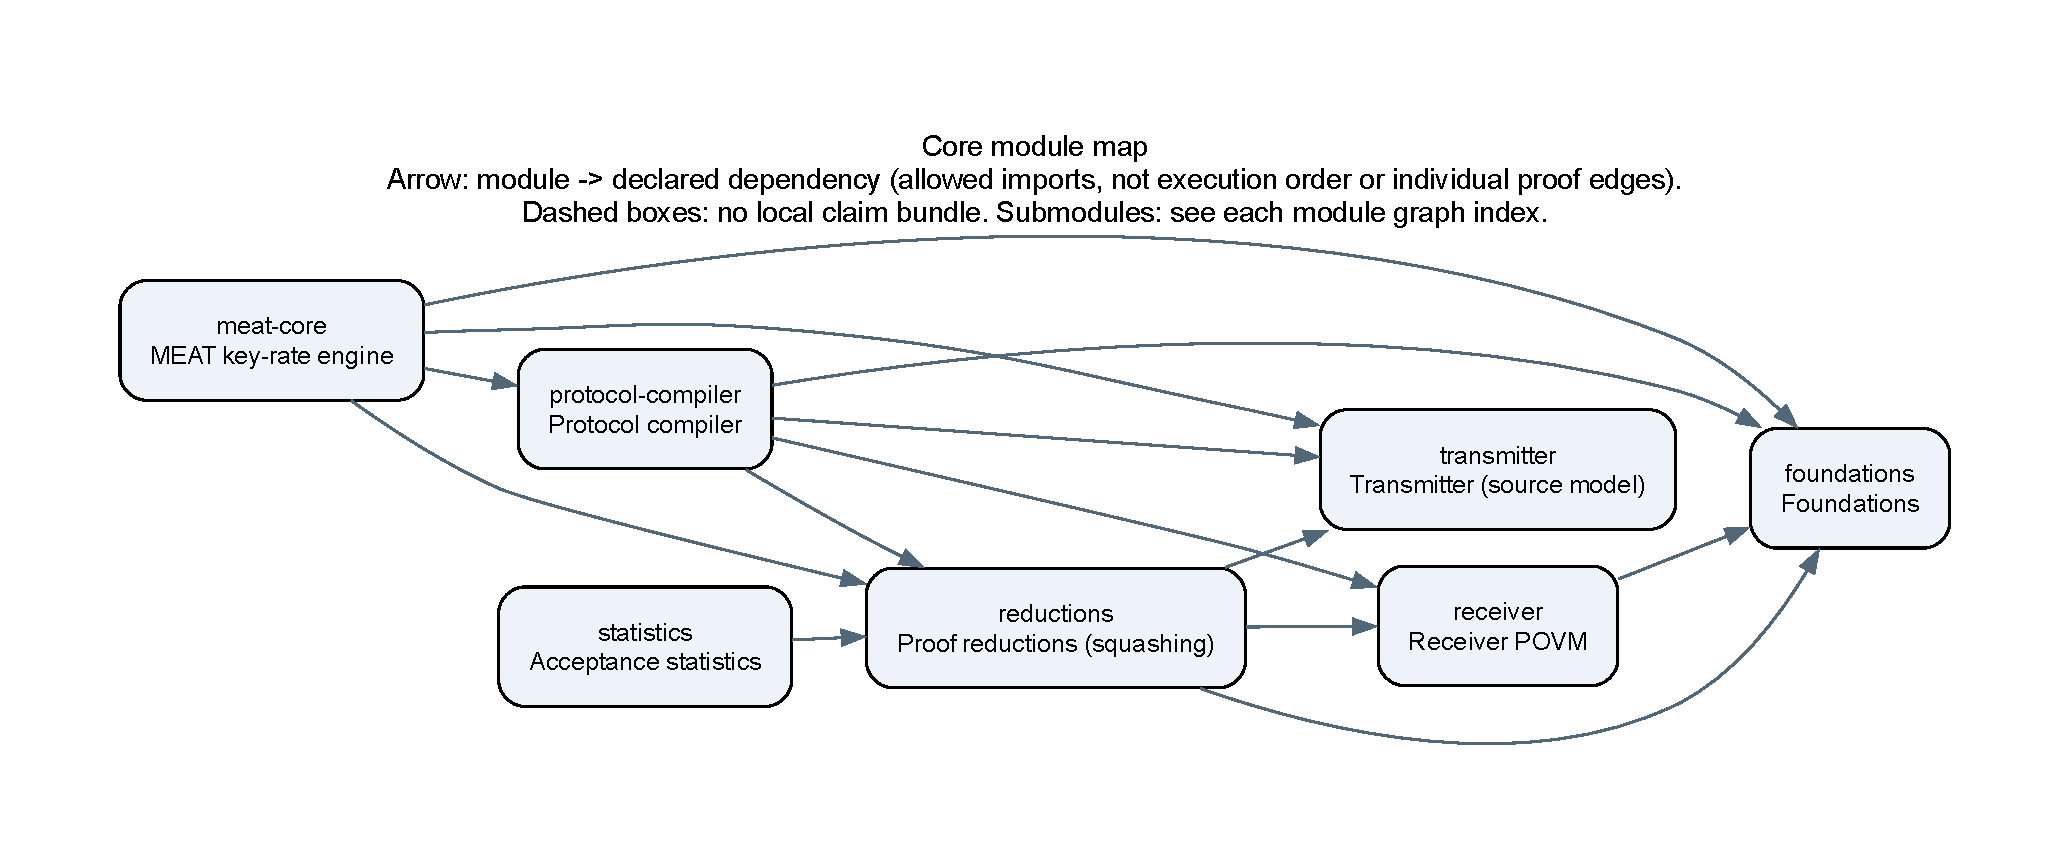
\includegraphics[width=\linewidth]{../module-graph.pdf}
